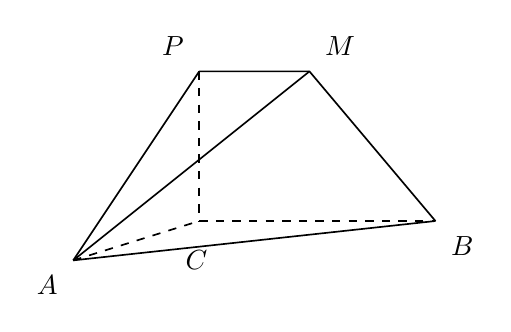
\begin{tikzpicture}[line width=0.6pt, >=stealth]
\coordinate (A) at (0,0);
\coordinate (C) at (1.6,0.5);
\coordinate (B) at (4.6,0.5);
\coordinate (P) at (1.6,2.4);
\coordinate (M) at (3.0,2.4);
% trapezoid PCBM: PM solid, BM solid, CB dashed, PC dashed
\draw (P) -- (M) -- (B);
\draw (P) -- (A);
\draw (A) -- (M);
\draw[dashed] (A)--(C);
\draw[dashed] (P) -- (C);
\draw[dashed] (C) -- (B);
\draw (A)--(B);
% labels
\node[below left=2pt] at (A) {$A$};
\node[below=2pt,xshift=-1pt,yshift=-5pt] at (C) {$C$};
\node[below right=2pt] at (B) {$B$};
\node[above left=2pt] at (P) {$P$};
\node[above right=2pt] at (M) {$M$};
\end{tikzpicture}
